\documentclass[letterpaper,11pt]{article}
\usepackage[spanish]{babel}
\usepackage[utf8]{inputenc}
\usepackage{graphicx}
\usepackage{amsfonts,amsmath,amssymb,float, amsthm,mathrsfs}  
\usepackage[right=4.5cm,left=2cm,top=3cm,bottom=3cm,headsep= 0.7cm,footskip=0.5cm]{geometry}
\usepackage{enumerate}
\usepackage{wrapfig} 
\usepackage[rflt]{floatflt} 
\usepackage{framed}
%\usepackage[most]{tcolorbox}
\usepackage[dvipsnames]{xcolor}
\colorlet{shadecolor}{green!20}
\setlength\FrameSep{0.5ex}
\usepackage{thmtools}
\usepackage{esint}
\usepackage{cancel}
\usepackage{listings} 
\usepackage{pstricks, caption}
\usepackage[colorlinks]{hyperref}
\usepackage{csquotes}
\usepackage{fullpage}
\usepackage{enumitem}
\usepackage{etoolbox}
\usepackage{tikz}
\usepackage{tikz-3dplot}
\tdplotsetmaincoords{80}{70}
\usetikzlibrary{decorations.markings}
\usetikzlibrary{arrows,babel}
\usepackage[font=small]{caption}
\usepackage{scalerel} %\scaleto{text}{size}
\usepackage{subfigure}
\usepackage{fancyhdr}
\usepackage{comment}
\usepackage{marginnote}
\usepackage{tensor}
\usepackage{cleveref}
\newcommand{\dbar}{\mathchar'26\mkern-12mu d}
\renewcommand*{\marginnotevadjust}{-0.1cm}
\renewcommand*{\marginfont}{\footnotesize}
\setlength{\headheight}{15pt}
\addtolength{\topmargin}{-14.49998pt}
\setlength{\headsep}{15pt}
\setlength{\footskip}{14.49998pt}
\decimalpoint
\newcommand{\grad}{^\circ}
\newlength{\drop}
\DeclareMathOperator{\sign}{sgn}
\DeclareMathOperator{\Log}{Log}
\providecommand{\norm}[1]{\lVert#1\rVert}

\let\cancelorigcolor\CancelColor% Just for conveniency...

\newcommand{\CancelTo}[3][]{%
  \ifblank{#1}{}{%
    \renewcommand{\CancelColor}{#1}%
  }
  \cancelto{#2}{#3}% 
}


\begin{document}

\pagestyle{plain}

\begin{flushleft}\vspace{-2cm}
Departamento de Física \\
Facultad de Cs. Físicas y Matemáticas\\
Universidad de Concepción
\end{flushleft}

\begin{flushright}\vspace{-1.5cm}
\textbf{Tópicos en Relatividad General} 
\end{flushright}



\rule{\linewidth}{0.1mm}

\begin{center}
\textbf{\LARGE Semana 9}
\end{center}

\begin{flushleft}
\textbf{Nombre:} Alejandro Saavedra San Martín. \\
\textbf{Profesor:} Guillermo Rubilar Alegría.
\end{flushleft}

\section*{Agujeros Negros}

\subsection*{Singularidades y radio de Schwarzschild}

Estudiaremos la estructura de la solución de Schwarzschild en regiones cercanas al \textit{radio de Schwarzschild}, donde el campo gravitacional es muy intenso. La geometría del espaciotiempo de Schwarzschild, en coordenadas de curvatura, es
\colorlet{shadecolor}{red!20}
\begin{shaded}
\begin{equation} \label{eq:Scwarzschild-metric}
    ds^2 = \left( 1 - \frac{2m}{r}\right) c^2 dt^2 - \frac{dr^2}{\left( 1- \frac{2m}{r} \right)} - r^2 \left[ d\theta^2 + \sin^2 \theta d\varphi^2 \right].
\end{equation}
    
\end{shaded}

Notemos que para $r \to 0$, $g_{00} \to - \infty$ y $g_{11} \to 0$, y para $r \to 2m^{+}$, $g_{00} \to 0$ y $g_{11} \to -\infty$, es decir, la métrica, en estas coordenadas, tiene un mal comportamiento cerca de $r = 0$ y $r = 2m$. Para comprobar si son singularidades de coordenadas o de curvatura, calculemos el siguiente escalar:
\begin{equation}
R_{\mu\nu\rho\sigma} R^{\mu\nu\rho\sigma}. 
\end{equation} 

En el siguiente \href{https://github.com/AleSaa66/Topicos-RG/blob/main/Semana%209/Semana-9.ipynb}{notebook} se encuentra que las únicas componentes no nulas del tensor de Riemann con todos los índices contravariantes y covariantes, respectivamente, son
\begingroup
\allowdisplaybreaks
\begin{align}
R^{0101} &= - R^{0110} = \frac{2m}{r^3}, \\
R^{0202} &= - R^{0220} = \frac{m}{r^4(2m - r)}, \\
R^{0303} &= - R^{0330} = \frac{m}{r^4(2m - r)\sin^2(\theta)}, \\
R^{1001} &= - R^{1010} = - \frac{2m}{r^3}, \\
R^{1212} &= - R^{1221} = - \frac{m(2m-r)}{r^6}, \\
R^{1313} &= - R^{1331} = - \frac{m(2m-r)}{r^6\sin^2(\theta)}, \\
R^{2002} &= - R^{2020} = - \frac{m}{r^4(2m-r)}, \\
R^{2112} &= - R^{2121} = \frac{m(2m-r)}{r^6}, \\
R^{2323} &= - R^{2332} = - \frac{2m}{r^7\sin^2(\theta)}, \\
R^{3003} &= - R^{3030} = - \frac{m}{r^4(2m-r)\sin^2(\theta)}, \\
R^{3113} &= - R^{3131} = \frac{m(2m-r)}{r^6\sin^2(\theta)}, \\
R^{3223} &= - R^{3232} = \frac{2m}{r^7\sin^2(\theta)}.
\end{align}
\endgroup

\begin{align}
R_{0101} &= - R_{0110} = \frac{2m}{r^3}, \\
R_{0202} &= - R_{0220} = \frac{m(2m-r)}{r^2}, \\
R_{0303} &= - R_{0330} = \frac{m(2m-r)\sin^2(\theta)}{r^2}, \\
R_{1001} &= - R_{1010} = - \frac{2m}{r^3}, \\
R_{1212} &= - R_{1221} = - \frac{m}{2m - r}, \\
R_{1313} &= - R_{1331} = - \frac{m \sin^2(\theta)}{2m-r}, \\
R_{2002} &= - R_{2020} =  - \frac{m(2m-r)}{r^2}, \\
R_{2112} &= - R_{2121} = \frac{m}{2m-r}, \\
R_{2323} &= - R_{2332} = - 2m r \sin^2(\theta), \\
R_{3003} &= - R_{3030} = - \frac{m(2m-r)\sin^2(\theta)}{r^2}, \\
R_{3113} &= - R_{3131} = \frac{m \sin^2(\theta)}{2m-r}, \\
R_{3223} &= - R_{3232} = 2mr \sin^2(\theta).
\end{align}

Entonces, 
\begin{equation}
R_{\mu\nu\rho\sigma} R^{\mu\nu\rho\sigma} = R_{0\nu\rho\sigma}R^{0\nu\rho\sigma} + R_{1\nu\rho\sigma} R^{1\nu\rho\sigma} + R_{2\nu\rho\sigma} R^{2\nu\rho\sigma} + R_{3\nu\rho\sigma} R^{3\nu\rho\sigma}. \label{eq:BH-1}
\end{equation} 

Desarrollando término a término:
\begin{align}
R_{0\nu\rho\sigma}R^{0\nu\rho\sigma} &= \CancelTo[\color{red}]{0}{R_{00\rho\sigma}R^{00\rho\sigma}} + R_{01\rho\sigma}R^{01\rho\sigma} + R_{02\rho\sigma}R^{02\rho\sigma} + R_{03\rho\sigma}R^{03\rho\sigma} \nonumber \\
&= R_{0101} R^{0101} + R_{0110} R^{0110} +  R_{0202} R^{0202} + R_{0220} R^{0220} + R_{0303} R^{0303} + R_{0330} R^{0330}  \nonumber \\
&=  2 R_{0101} R^{0101} + 2 R_{0202} R^{0202} + 2 R_{0303} R^{0303} \nonumber \\
&= 2 \left(\frac{2m}{r^3}\right)^2 + 2 \frac{m(2m-r)}{r^2} \frac{m}{r^4(2m-r)} + 2 \frac{m(2m-r)\sin^2(\theta)}{r^2} \frac{m}{r^4(2m-r)\sin^2(\theta)} \nonumber \\
&= \frac{8m^2}{r^6} + \frac{2m^2}{r^6} + \frac{2m^2}{r^6} \nonumber\\
&= \frac{12m^2}{r^6}. \label{eq:BH-2}
\end{align}

\begin{align}
R_{1\nu\rho\sigma}R^{1\nu\rho\sigma} &= R_{10\rho\sigma}R^{10\rho\sigma} + \CancelTo[\color{red}]{0}{R_{11\rho\sigma}R^{11\rho\sigma}} + R_{12\rho\sigma}R^{12\rho\sigma} + R_{13\rho\sigma}R^{13\rho\sigma} \nonumber \\
&= R_{1001} R^{1001} + R_{1010} R^{1010} +  R_{1212} R^{1212} + R_{1221} R^{1221} + R_{1313} R^{1313} + R_{1331} R^{1331}  \nonumber \\
&=  2  R_{1001} R^{1001} + 2 R_{1212} R^{1212} + 2 R_{1313} R^{1313} \nonumber \\
&= 2 \left(\frac{2m}{r^3}\right)^2 + 2 \frac{m}{2m-r} \frac{m(2m-r)}{r^6} + 2 \frac{m \sin^2(\theta)}{2m-r} \frac{m(2m-r)}{r^6\sin^2(\theta)} \nonumber \\
&= \frac{8m^2}{r^6} + \frac{2m^2}{r^6} + \frac{2m^2}{r^6} \nonumber\\
&= \frac{12m^2}{r^6}. \label{eq:BH-3}
\end{align}

\begin{align}
R_{2\nu\rho\sigma}R^{2\nu\rho\sigma} &= R_{20\rho\sigma}R^{20\rho\sigma} + R_{21\rho\sigma}R^{21\rho\sigma} + \CancelTo[\color{red}]{0}{R_{22\rho\sigma}R^{22\rho\sigma}} + R_{23\rho\sigma}R^{23\rho\sigma} \nonumber \\
&= R_{2002} R^{2002} + R_{2020} R^{2020} +  R_{2112} R^{2112} + R_{2121} R^{2121} + R_{2323} R^{2323} + R_{2332} R^{2332}  \nonumber \\
&=  2  R_{2002} R^{2002} + 2 R_{2112} R^{2112} + 2 R_{2323} R^{2323} \nonumber \\
&= 2 \frac{m(2m-r)}{r^2} \frac{m}{r^4(2m-r)} + 2 \frac{m}{2m-r} \frac{m(2m-r)}{r^6} + 2 \left(2mr\sin^2(\theta)\right) \frac{2m}{r^7\sin^2(\theta)} \nonumber \\
&= \frac{2m^2}{r^6} + \frac{2m^2}{r^6} + \frac{8 m^2}{r^6} \nonumber\\
&= \frac{12m^2}{r^6}. \label{eq:BH-4}
\end{align}

\begin{align}
R_{3\nu\rho\sigma}R^{3\nu\rho\sigma} &= R_{30\rho\sigma}R^{30\rho\sigma} + R_{31\rho\sigma}R^{31\rho\sigma} + R_{32\rho\sigma}R^{32\rho\sigma} + \CancelTo[\color{red}]{0}{R_{33\rho\sigma}R^{33\rho\sigma}} \nonumber \\
&= R_{3003} R^{3003} + R_{3030} R^{3030} +  R_{3113} R^{3113} + R_{3131} R^{3131} + R_{3223} R^{3223} + R_{3233} R^{3232}  \nonumber \\
&=  2  R_{3003} R^{3003} + 2 R_{3113} R^{3113} + 2 R_{3223} R^{3223} \nonumber \\
&= 2 \frac{m(2m-r)\sin^2(\theta)}{r^2} \frac{m}{r^4(2m-r)\sin^2(\theta)} + 2 \frac{m \sin^2(\theta)}{2m-r} \frac{m(2m-r)}{r^6 \sin^2(\theta)} + 2 \left(2mr\sin^2(\theta)\right) \frac{2m}{r^7\sin^2(\theta)} \nonumber \\
&= \frac{2m^2}{r^6} + \frac{2m^2}{r^6} + \frac{8 m^2}{r^6} \nonumber\\
&= \frac{12m^2}{r^6}. \label{eq:BH-5}
\end{align}

Reemplazando \eqref{eq:BH-2}-\eqref{eq:BH-5} en \eqref{eq:BH-1}, obtenemos que
\colorlet{shadecolor}{green!20}
\begin{shaded}
\begin{equation}
R_{\mu\nu\rho\sigma} R^{\mu\nu\rho\sigma} = \frac{48m^2}{r^6},
\end{equation}
\end{shaded}
lo que prueba que $r = 0$ (el origen del sistema coordenada usado) representa una singularidad de la geometría, donde la curvatura diverge. Sin embargo, en $r = 2m$ no diverge. De hecho ninguno de los invariantes diverge en $r = 2m$, por ejemplo, el escalar de curvatura $R = 0$. Por lo tanto, la esfera definida por $r = 2m$ no es una singularidad de curvatura. 

Del documento de la semana 6, tenemos que la dilatación temporal gravitacional está dada por
\begin{equation}
\frac{\Delta \tau_{\text{r}}}{\Delta \tau_{\text{e}}} = \sqrt{\frac{1 -  \frac{2m}{r_{\text{r}}}}{1 - \frac{2m}{r_{\text{e}}}}}.
\end{equation}

Notemos que en $r_{\text{e}} = 2m$, el cociente diverge. Ésta es la razón de porqué se dice que la superficie esférica en $r = 2m$ es una superficie infinitamente desplazada al rojo por efecto de la dilatación temporal gravitacional o una superficie de redshift infinito.

\subsection*{Diagrama Espacio-Temporal en Coordenadas de Schwarzschild}

Consideremos en particular curvas (geodésicas) radiales tipo luz, es decir, para las cuales $\theta$ y $\varphi$ son constantes y $ds^2 = 0$. Esta última condición se reduce a 
\begin{equation}
\left(1 - \frac{2m}{r}\right) c^2 dt^2 - \frac{dr^2}{\left(1 - \frac{2m}{r}\right)} = 0.
\end{equation}

Despejando $dt/dr$:
\begin{align}
c^2dt^2 &= \frac{dr^2}{\left(1 - \frac{2m}{r}\right)^2} \\
c \,dt &= \pm \frac{dr}{\sqrt{\left(1 - \frac{2m}{r}\right)^2}} \\
c\frac{dt}{dr} &= \pm \frac{1}{\left| 1 - \frac{2m}{r}\right|}.  \label{eq:BH-6}
\end{align}

Consideremos 
\begin{equation}
\int \frac{dr}{\left| 1 - \frac{2m}{r} \right|} = \int \frac{r}{|r-2m|} \,dr.
\end{equation} 

Para $r > 2m$, tenemos que
\begin{align}
\int \frac{r}{|r-2m|} \,dr &= \int \frac{r}{r - 2m} \,dr \nonumber\\
&= \int 1 + \frac{2m}{r - 2m} \,dr \nonumber \\
&= r + 2m \ln(r-2m) + C.
\end{align}

Por otro lado, si $r < 2m$, se tiene que
\begin{equation}
\int \frac{r}{|r-2m|} \,dr = - \int \frac{r}{r - 2m} \,dr = - r - 2m \ln|r-2m| + C.
\end{equation}

Entonces, si integramos entre $a$ y $b$, encontramos que
\begin{equation}
\int_a^b \frac{dr}{\left| 1 - \frac{2m}{r} \right|}  = \pm \left[ b - a + 2m\ln\left(\frac{b-2m}{a-2m}\right) \right], \quad a < b,
\end{equation}
donde el signo positivo y negativo corresponde a los casos en que $a,b > 2m$ y $a,b < 2m$, respectivamente. El logaritmo natural fue escrito sin valor absoluto, pues si $a,b > 2m$ o  $a,b < 2m$, el cociente siempre es positivo. De esta forma podemos integrar con respecto a $r$ la ecuación \eqref{eq:BH-6}.

Si $r > 2m$ el signo $+$ en \eqref{eq:BH-6} corresponde a fotones alejándose del centro de simetría y el signo $-$ a fotones acercándose a éste. En este caso, integrando de $t_0$ a $t$ en la coordenada temporal y de $r_0$ a $r$ en la coordenada radial, obtenemos
\begin{equation}
c(t - t_0) = r - r_0 + 2m \ln\left(\frac{r - 2m}{r_0 - 2m}\right),  \label{eq:BH-out}
\end{equation}
para fotones salientes, y
\begin{equation}
c(t - t_0) = r_0 - r - 2m \ln\left(\frac{r - 2m}{r_0 - 2m}\right),  \label{eq:BH-in}
\end{equation}
para fotones entrantes, que pasan por el evento con coordenadas $(ct_0,r_0)$, respectivamente. En la figura \ref{fig:Null-Curves-Sch} se pueden observar curvas nulas radiales en coordenadas de curvatura salientes y entrantes.

\begin{figure}
\centering
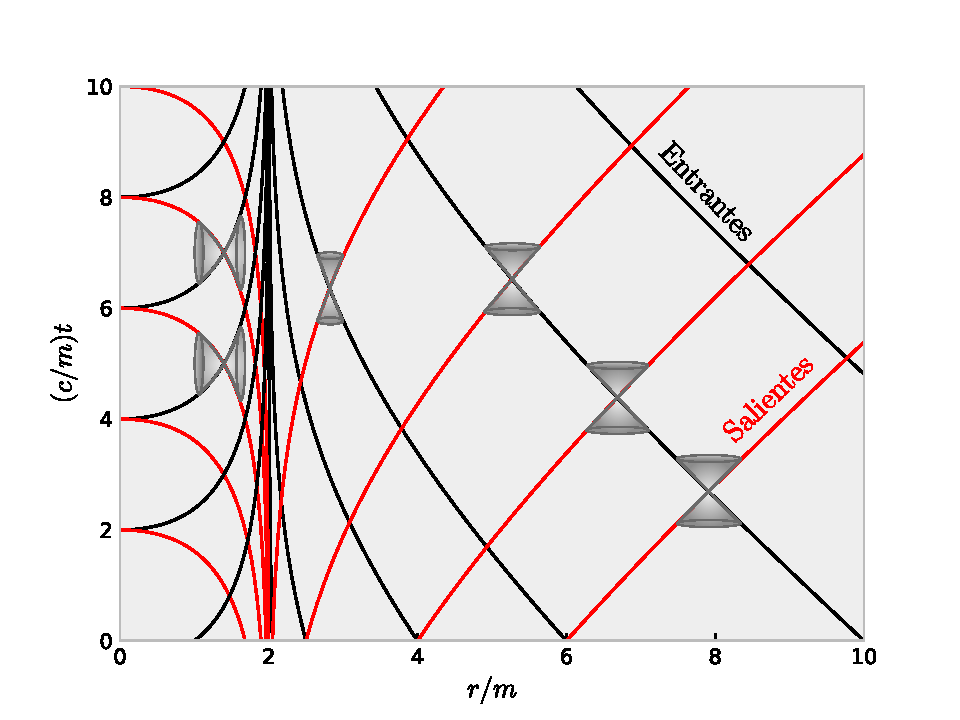
\includegraphics[scale=0.7]{Fig-Curvas-Nulas-Schwarzschild}
\caption{Curvas nulas radiales en coordenadas de curvatura.}
\label{fig:Null-Curves-Sch}
\end{figure}

Observando la figura \ref{fig:Null-Curves-Sch} o la ecuación \eqref{eq:BH-6}, podemos concluir que muy lejos del centro de fuerzas $r \gg 2m$, recobramos
\begin{equation}
\frac{dr}{dt} = \pm c,
\end{equation}
tal como en un espaciotiempo plano. Por otro lado, cuando $r$ se aproxima a $2m$ (por ``la derecha"), tenemos
\begin{equation}
\frac{dt}{dr} \to \pm \infty,
\end{equation}
y los conos de luz se ``cierran", ya que las líneas tienden a ser paralelas al eje $t$. Esto tendrá como consecuencia que al acercarse a $r = 2m$ la coordenada temporal de la trayectoria del fotón aumentará indefinidamente.

Para describir cómo se ``ve" la caída del fotón desde lejos, consideremos un observador en reposo en $r = R > 2m$, un fotón cayendo hacia la singularidad, y dos eventos $E_1$ y $E_2$ en su línea de mundo, con coordenadas $(ct,r) = (ct_1,r_1)$ y $(ct,r) = (ct_2,r_2)$, respectivamente, con $r_2 < r_1 < R$, ver figura \ref{fig:Photon-Falss}. De acuerdo a la ecuación \eqref{eq:BH-in}, las coordenadas de estos eventos están relacionadas por medio de
\begin{align}
c(t_2 - t_1) &= r_1 - r_2 - 2m \ln\left(\frac{r_2 - 2m}{r_1 - 2m}\right) \nonumber\\
&= r_1 - r_2 + 2m \ln\left(\frac{r_1 - 2m}{r_2 - 2m}\right). \label{eq:BH-7}
\end{align}

\begin{figure}
\centering
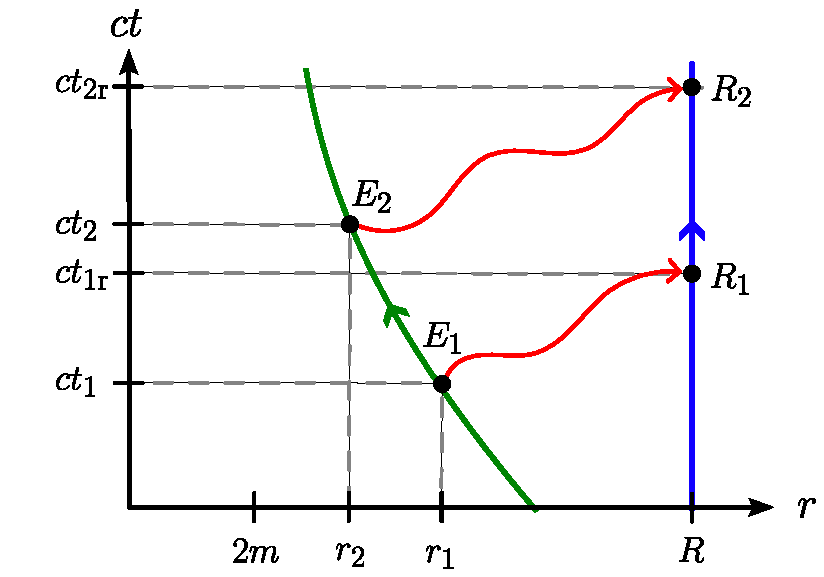
\includegraphics[scale=0.7]{Fig-Caida-Foton}
\caption{Caída de un fotón.}
\label{fig:Photon-Falss}
\end{figure}

Consideremos que cuando el fotón pasa por el evento $E_1$ una señal luminosa (otro fotón) es enviado hacia el observador. Este nuevo fotón viaja desde el evento $E_1$ hasta el evento de recepción $R_1$, con coordenadas $(ct,r) = (ct_{1\text{r}},R)$. Como estos eventos pertenecen a la línea de mundo de un fotón alejándose de la singularidad, usamos \eqref{eq:BH-out} para encontrar la relación entre sus coordenadas:
\begin{equation}
c(t_{1\text{r}} -t_1) = R - r_1 + 2m \ln\left(\frac{R-2m}{r_1 - 2m}\right). \label{eq:BH-8}
\end{equation}

Similarmente, si en el evento $E_2$ se emite una segunda señal luminosa hasta el observador, de modo que éste la recibe en el evento $R_2$ con coordenadas $(ct,r) = (ct_{2\text{r}},R)$, entonces
\begin{equation}
c(t_{2\text{r}} -t_2) = R - r_2 + 2m \ln\left(\frac{R-2m}{r_2 - 2m}\right). \label{eq:BH-9}
\end{equation}

El intervalo de coordenada temporal entre la recepción de las dos señales por el observador en reposo en la posición $r = R$ está dado por $(\Delta t)_{\text{r}} = t_{2\text{r}} - t_{1\text{r}}$. Si a la ecuación \eqref{eq:BH-9} le restamos la ecuación \eqref{eq:BH-8}, obtenemos que
\begin{align}
c(t_{2\text{r}} - t_{1\text{r}}) - c (t_2 - t_1) &= r_1 - r_2 + 2m \ln\left( \frac{R-2m}{r_2 - 2m} \frac{r_1 - 2m}{R-2m}\right) \\
c(\Delta t)_{\text{r}} &=  c (t_2 - t_1) + r_1 - r_2 + 2m \ln\left( \frac{r_1 - 2m}{r_2 - 2m} \right).
\end{align}

Usando la ecuación \eqref{eq:BH-7}, encontramos
\colorlet{shadecolor}{green!20}
\begin{shaded}
\begin{equation}
c(\Delta t)_{\text{r}} = 2 \left[ r_1 - r_2 + 2m \ln\left( \frac{r_1 - 2m}{r_2 - 2m} \right) \right].
\end{equation}
\end{shaded}

Por otro lado, el tiempo (propio) medido por el observador en $r = R$ entre las dos señales es 
\begin{equation}
(\Delta \tau)_{\text{r}} = \sqrt{g_{00}} (\Delta t)_{\text{r}} = (\Delta t)_{\text{r}} \sqrt{1 - \frac{2m}{R}}.
\end{equation}

Para un observador en el infinito, tendremos $(\Delta \tau)_{\text{r}}  = (\Delta t)_{\text{r}}$. Como consecuencia, desde el punto de vista de un observador externo (en $r = R$, o en el infinito) el fotón requiere un tiempo infinito en llegar a $r = 2m$, es decir, el observador nunca registra que 
el fotón cruza el horizonte, sino que lo observa acercarse cada vez más lentamente.

\subsection*{Coordenadas de Eddington-Finkelstein}

Consideremos nuevas coordenadas $\bar{x}^{\mu} = (c\bar{t},r,\theta,\varphi)$ tales que 
\begin{equation}
\bar{t}(t,r) := t + \frac{2m}{c} \ln|r - 2m|, \label{eq:Coor-EF}
\end{equation}
conocida como la \textbf{coordenada de Eddington-Finkelstein retardada}.

La trayectoria de un fotón entrante puede re-escribirse como
\begin{equation}
\left[ ct + 2m \ln\left(r-2m\right)\right] - \left[ct_0 + 2m \ln\left(r_0-2m\right) \right] = r_0 - r. 
\end{equation}

Usando la transformación de coordenadas \eqref{eq:Coor-EF}, encontramos que la trayectoria del fotón entrante en estas nuevas coordenadas es
\begin{equation}
c(\bar{t} - \bar{t}_0) = r_0 - r, \label{eq:EF-in}
\end{equation}
que en el plano $(c\bar{t},r)$ corresponde precisamente una línea recta con pendiente $-1$ (45 grados respecto al eje $r$).

Determinemos el diferencial de \eqref{eq:Coor-EF}:
\begin{align}
d\bar{t} &= dt + \frac{2m}{c} \frac{1}{|r - 2m|} \frac{d}{dr}(|r - 2m|) dr \nonumber \\
&= dt + \frac{2m}{c} \frac{1}{|r - 2m|} \frac{|r - 2m|}{r-2m} dr \nonumber \\
&= dt + \frac{2m}{c} \frac{dr}{r - 2m}. 
\end{align}

Reemplazando en la métrica \eqref{eq:Scwarzschild-metric}, obtenemos que
\begingroup
\allowdisplaybreaks
\begin{align}
ds^2 &= \left( 1 - \frac{2m}{r}\right) c^2 \left(d\bar{t} - \frac{2m}{c} \frac{dr}{r - 2m} \right)^2 - \frac{dr^2}{\left( 1- \frac{2m}{r} \right)} - r^2 \left[ d\theta^2 + \sin^2 \theta d\varphi^2 \right] \nonumber \\
&= c^2 \frac{(r - 2m)}{r}  \left(d\bar{t}^2 - \frac{4m}{c} \frac{d\bar{t} \, dr}{r - 2m} + \frac{4m^2}{c^2} \frac{dr^2}{(r-2m)^2} \right) - \frac{dr^2}{\left( 1- \frac{2m}{r} \right)} - r^2 \left[ d\theta^2 + \sin^2 \theta d\varphi^2 \right] \nonumber \\
&= \left(1 - \frac{2m}{r}\right) c^2d\bar{t}^2 - \frac{4m}{r} c \, d\bar{t} \, dr + \left[\frac{4m^2}{r(r-2m)} - \frac{r}{r-2m} \right] dr^2 - r^2 \left[ d\theta^2 + \sin^2 \theta d\varphi^2 \right]\nonumber  \\
&= \left(1 - \frac{2m}{r}\right) c^2d\bar{t}^2 - \frac{4m}{r} c \, d\bar{t} \, dr + \left[\frac{4m^2 - r^2}{r(r-2m)}\right] dr^2 - r^2 \left[ d\theta^2 + \sin^2 \theta d\varphi^2 \right]\nonumber  \\
&= \left(1 - \frac{2m}{r}\right) c^2d\bar{t}^2 - \frac{4m}{r} c \, d\bar{t} \, dr - \left[\frac{r + 2m}{r}\right] dr^2 - r^2 \left[ d\theta^2 + \sin^2 \theta d\varphi^2 \right] \nonumber  \\
&= \left(1 - \frac{2m}{r}\right) c^2d\bar{t}^2 - \frac{4m}{r} c \, d\bar{t} \, dr - \left(1 + \frac{2m}{r}\right) dr^2 - r^2 \left(d\theta^2 + \sin^2\theta d\varphi^2\right).
\end{align}
\endgroup

Por lo tanto, en términos de las nuevas coordenadas $\bar{x}^{\mu}$, el elemento de línea adopta la forma
\colorlet{shadecolor}{green!20}
\begin{shaded}
\begin{equation}
ds^2 = \left(1 - \frac{2m}{r}\right) c^2d\bar{t}^2 - \frac{4m}{r} c \, d\bar{t} \, dr - \left(1 + \frac{2m}{r}\right) dr^2 - r^2 \left(d\theta^2 + \sin^2\theta d\varphi^2\right).
\end{equation}
\end{shaded}

Para encontrar una relación similar a \eqref{eq:EF-in}, pero para fotones salientes, escribamos 
\begin{align}
c(t- t_0) &= r - r_0 + 2m\ln\left(\frac{r - 2m}{r_0 - 2m}\right) \\
ct - ct_0 + 2m\ln\left(\frac{r - 2m}{r_0 - 2m}\right) &= r - r_0 + 2m\ln\left(\frac{r - 2m}{r_0 - 2m}\right) + 2m\ln\left(\frac{r - 2m}{r_0 - 2m}\right) \\
\left[ ct + 2m\ln(r-2m)\right] - \left[ct_0 + 2m \ln(r_0 - 2m)\right] &= r - r_0  + 4m\ln\left(\frac{r - 2m}{r_0 - 2m}\right).
\end{align}

Usando la transformación de coordenadas \eqref{eq:Coor-EF}, encontramos que la trayectoria del fotón saliente en estas nuevas coordenadas es
\begin{equation}
c(\bar{t} - \bar{t}_0) = r - r_0 + 4m \ln \left| \frac{r-2m}{r_0 - 2m} \right|.
\end{equation}

En la figura \ref{fig:Null-Curves-EF} se pueden observar curvas nulas radiales en coordenadas de Eddington-Finkelstein salientes y entrantes. Note que la superficie $r = 2m$ sólo permite cruzar a partículas cayendo hacia la singularidad central, sin posibilidad de salir (el cono de luz futuro se inclina hacia la región para $r < 2m$). Las líneas de mundo entrantes cruzan desde la región externa hacia la interna sin problemas (no como en el caso usando coordenadas de Schwarzschild).

\begin{figure}
\centering
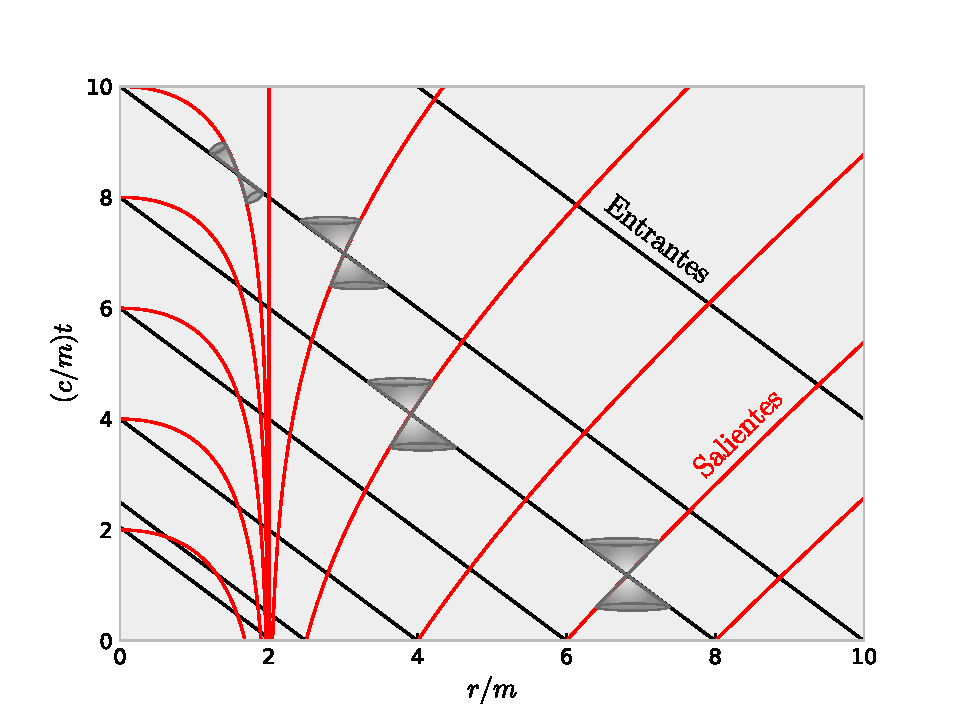
\includegraphics[scale=0.7]{Fig-Curvas-Nulas-Eddington-Finkelstein}
\caption{Curvas nulas radiales en coordenadas de Eddington-Finkelstein.}
\label{fig:Null-Curves-EF}
\end{figure}

\subsection*{Partículas cayendo radialmente}

Consideremos la trayectoria de una partícula cayendo libremente en un movimiento radial hacia la singularidad. La trayectoria es entonces una geodésica radial tipo tiempo. De acuerdo a lo discutido en el documento de la semana 2, la trayectoria tiene como constantes de movimiento a $k$ y $h$ dadas por
\begin{equation}
k = \left( 1  - \frac{2m}{r}\right) \dot{t}, \quad hmc = r^2\sin^2\theta \dot{\varphi}, \label{eq:particle-fall-1}
\end{equation}
con $h = 0$, pues como la partícula cae libremente $\dot{\varphi}(0) = 0$. Nos centraremos en las trayectorias correspondientes a partículas que caen ``desde el reposo en el infinito", es decir, tal que $\dot{r} \to 0$ cuando $r \to \infty$. 

Recordemos que la dinámica radial estaba dada por la ecuación
\begin{equation}
\dot{r}^2 = k^2c^2 - c^2 \left(1 - \frac{2m}{r} \right)\left( 1 + \frac{h^2m^2}{r^2}\right). \label{eq:particle-fall-2}
\end{equation}

Evaluando para $r \to \infty$, obtenemos que
\begin{equation}
0 = k^2c^2 - c^2 \Rightarrow k^2 = 1. \label{eq:particle-fall-3}
\end{equation}

Usando la primera ecuación de \eqref{eq:particle-fall-1}, para las trayectorias ``orientadas hacia el futuro", $k = 1$. Con todo ésto, la ecuación \eqref{eq:particle-fall-2} nos queda
\begin{align}
\dot{r}^2 &= k^2c^2 - c^2 \left(1 - \frac{2m}{r} \right)\left( 1 + \cancelto{0}{\frac{h^2m^2}{r^2}}\quad \right) \\
\dot{r}^2 &= c^2 - c^2\left(1 - \frac{2m}{r} \right) \\
\dot{r}^2 &= \frac{2mc^2}{r}. \label{eq:particle-fall-4}
\end{align}

Como estamos considerando una partícula acercándose a la singularidad central, al tomar la raíz cuadrada a ambos lados de la ecuación \eqref{eq:particle-fall-4}, nos quedamos con el resultado con el signo negativo, ésto es,
\begin{equation}
\frac{dr}{d\tau} = - c \sqrt{\frac{2m}{r}}. \label{eq:particle-fall-5}
\end{equation}

Integrando la expresión \eqref{eq:particle-fall-5}:
\begin{align}
c \int_{\tau_0}^{\tau} d\tau' &= - \int_{r_0}^{r} \sqrt{\frac{r'}{2m}} dr' \\
c (\tau - \tau_0) &=  \left. - \frac{2}{3\sqrt{2m}} r' \right|_{r_0}^{r} \\
c (\tau - \tau_0) &=  \frac{2}{3\sqrt{2m}} \left( r_0^{3/2} - r^{3/2}\right),
\end{align}
donde $\tau_0$ es el tiempo propio registrado en el instante en que éste pasa por $r = r_0$. Como consecuencia, el intervalo de tiempo propio desde que la partícula cruza $r =r_0$ y que llega a la singularidad central es finito
\begin{equation}
c(\tau|_{r = 0} - \tau_0) = \frac{2}{3\sqrt{2m}} r_0^{3/2}.
\end{equation}

En particular, el tiempo propio requerido para caer desde el horizonte $(r_0 = 2m)$ hasta la singularidad central es
\begin{equation}
\Delta \tau = \frac{2}{3c \sqrt{2m}} (2m)^{3/2} = \frac{2}{3c} \sqrt{\frac{8m^3}{2m}} = \frac{4m}{3c}.
\end{equation}

Para analizar cómo varía la coordenada $t$ en este proceso, calculemos
\begin{equation}
c \frac{dt}{dr} = c \frac{dt}{d\tau} \frac{d\tau}{dr} = c \frac{\dot{t}}{\dot{r}}. \label{eq:particle-fall-6}
\end{equation}

Reemplazando \eqref{eq:particle-fall-1} (para $k = 1$) y \eqref{eq:particle-fall-5} en \eqref{eq:particle-fall-6}:
\begin{equation}
c \frac{dt}{dr} = - \frac{c}{\left( 1 - \frac{2m}{r}\right)}  \frac{1}{c}\sqrt{\frac{r}{2m}} = - \frac{1}{1 - \frac{2m}{r}} \sqrt{\frac{r}{2m}}. \label{eq:particle-fall-7}
\end{equation}

Si calculamos la integral, ver  el \href{https://github.com/AleSaa66/Topicos-RG/blob/main/Semana%209/Semana-9.ipynb}{notebook}, obtenemos que
\begin{equation}
\int \frac{1}{1 - \frac{2m}{r}} \sqrt{\frac{r}{2m}} dr =  \frac{2}{3 \sqrt{2m}} \left(r^{3/2} +  6m \sqrt{r} \right) +  2m \ln\left( \frac{\sqrt{r} - \sqrt{2m}}{\sqrt{r} + \sqrt{2m}}\right) + C, 
\end{equation}
donde $C$ es una constante de integración. Entonces, integrando la ecuación \eqref{eq:particle-fall-7}, con respecto a $r$
\begin{align}
c\int_{t_0}^{t} dt' &=  - \int_{r_0}^{r} \frac{1}{1 - \frac{2m}{r'}} \sqrt{\frac{r'}{2m}} dr' \\
c(t - t_0) &= \left[-\frac{2}{3 \sqrt{2m}} \left(r'^{3/2} +  6m \sqrt{r'} \right) -  2m \ln\left( \frac{\sqrt{r'} - \sqrt{2m}}{\sqrt{r'} + \sqrt{2m}}\right)\right]_{r_0}^{r} \\
c(t - t_0) &= - \frac{2}{3\sqrt{2m}} \left( r^{3/2} +  6m \sqrt{r} - r_0^{3/2} -  6m \sqrt{r_0} \right) -  2m \ln\left( \frac{\sqrt{r} - \sqrt{2m}}{\sqrt{r} + \sqrt{2m}}\right) + 2m \ln\left( \frac{\sqrt{r_0} - \sqrt{2m}}{\sqrt{r_0} + \sqrt{2m}}\right) \\
c(t - t_0) &= - \frac{2}{3\sqrt{2m}} \left( r^{3/2} - r_0^{3/2} +  6m \sqrt{r}  -  6m \sqrt{r_0} \right) + 2m \ln\left[\frac{\left(\sqrt{r} + \sqrt{2m}\right)\left(\sqrt{r_0} - \sqrt{2m}\right)}{\left(\sqrt{r} - \sqrt{2m}\right)\left(\sqrt{r_0} + \sqrt{2m}\right)}\right].
\end{align}

Vemos de esta expresión que la coordenada temporal de la trayectoria de la partícula crece
indefinidamente a medida que ésta se acerca al horizonte.

\end{document}

